% Options for packages loaded elsewhere
\PassOptionsToPackage{unicode}{hyperref}
\PassOptionsToPackage{hyphens}{url}
\PassOptionsToPackage{dvipsnames,svgnames,x11names}{xcolor}
%
\documentclass[
  letterpaper,
  DIV=11,
  numbers=noendperiod]{scrartcl}

\usepackage{amsmath,amssymb}
\usepackage{iftex}
\ifPDFTeX
  \usepackage[T1]{fontenc}
  \usepackage[utf8]{inputenc}
  \usepackage{textcomp} % provide euro and other symbols
\else % if luatex or xetex
  \usepackage{unicode-math}
  \defaultfontfeatures{Scale=MatchLowercase}
  \defaultfontfeatures[\rmfamily]{Ligatures=TeX,Scale=1}
\fi
\usepackage{lmodern}
\ifPDFTeX\else  
    % xetex/luatex font selection
\fi
% Use upquote if available, for straight quotes in verbatim environments
\IfFileExists{upquote.sty}{\usepackage{upquote}}{}
\IfFileExists{microtype.sty}{% use microtype if available
  \usepackage[]{microtype}
  \UseMicrotypeSet[protrusion]{basicmath} % disable protrusion for tt fonts
}{}
\makeatletter
\@ifundefined{KOMAClassName}{% if non-KOMA class
  \IfFileExists{parskip.sty}{%
    \usepackage{parskip}
  }{% else
    \setlength{\parindent}{0pt}
    \setlength{\parskip}{6pt plus 2pt minus 1pt}}
}{% if KOMA class
  \KOMAoptions{parskip=half}}
\makeatother
\usepackage{xcolor}
\setlength{\emergencystretch}{3em} % prevent overfull lines
\setcounter{secnumdepth}{-\maxdimen} % remove section numbering
% Make \paragraph and \subparagraph free-standing
\ifx\paragraph\undefined\else
  \let\oldparagraph\paragraph
  \renewcommand{\paragraph}[1]{\oldparagraph{#1}\mbox{}}
\fi
\ifx\subparagraph\undefined\else
  \let\oldsubparagraph\subparagraph
  \renewcommand{\subparagraph}[1]{\oldsubparagraph{#1}\mbox{}}
\fi

\usepackage{color}
\usepackage{fancyvrb}
\newcommand{\VerbBar}{|}
\newcommand{\VERB}{\Verb[commandchars=\\\{\}]}
\DefineVerbatimEnvironment{Highlighting}{Verbatim}{commandchars=\\\{\}}
% Add ',fontsize=\small' for more characters per line
\usepackage{framed}
\definecolor{shadecolor}{RGB}{241,243,245}
\newenvironment{Shaded}{\begin{snugshade}}{\end{snugshade}}
\newcommand{\AlertTok}[1]{\textcolor[rgb]{0.68,0.00,0.00}{#1}}
\newcommand{\AnnotationTok}[1]{\textcolor[rgb]{0.37,0.37,0.37}{#1}}
\newcommand{\AttributeTok}[1]{\textcolor[rgb]{0.40,0.45,0.13}{#1}}
\newcommand{\BaseNTok}[1]{\textcolor[rgb]{0.68,0.00,0.00}{#1}}
\newcommand{\BuiltInTok}[1]{\textcolor[rgb]{0.00,0.23,0.31}{#1}}
\newcommand{\CharTok}[1]{\textcolor[rgb]{0.13,0.47,0.30}{#1}}
\newcommand{\CommentTok}[1]{\textcolor[rgb]{0.37,0.37,0.37}{#1}}
\newcommand{\CommentVarTok}[1]{\textcolor[rgb]{0.37,0.37,0.37}{\textit{#1}}}
\newcommand{\ConstantTok}[1]{\textcolor[rgb]{0.56,0.35,0.01}{#1}}
\newcommand{\ControlFlowTok}[1]{\textcolor[rgb]{0.00,0.23,0.31}{#1}}
\newcommand{\DataTypeTok}[1]{\textcolor[rgb]{0.68,0.00,0.00}{#1}}
\newcommand{\DecValTok}[1]{\textcolor[rgb]{0.68,0.00,0.00}{#1}}
\newcommand{\DocumentationTok}[1]{\textcolor[rgb]{0.37,0.37,0.37}{\textit{#1}}}
\newcommand{\ErrorTok}[1]{\textcolor[rgb]{0.68,0.00,0.00}{#1}}
\newcommand{\ExtensionTok}[1]{\textcolor[rgb]{0.00,0.23,0.31}{#1}}
\newcommand{\FloatTok}[1]{\textcolor[rgb]{0.68,0.00,0.00}{#1}}
\newcommand{\FunctionTok}[1]{\textcolor[rgb]{0.28,0.35,0.67}{#1}}
\newcommand{\ImportTok}[1]{\textcolor[rgb]{0.00,0.46,0.62}{#1}}
\newcommand{\InformationTok}[1]{\textcolor[rgb]{0.37,0.37,0.37}{#1}}
\newcommand{\KeywordTok}[1]{\textcolor[rgb]{0.00,0.23,0.31}{#1}}
\newcommand{\NormalTok}[1]{\textcolor[rgb]{0.00,0.23,0.31}{#1}}
\newcommand{\OperatorTok}[1]{\textcolor[rgb]{0.37,0.37,0.37}{#1}}
\newcommand{\OtherTok}[1]{\textcolor[rgb]{0.00,0.23,0.31}{#1}}
\newcommand{\PreprocessorTok}[1]{\textcolor[rgb]{0.68,0.00,0.00}{#1}}
\newcommand{\RegionMarkerTok}[1]{\textcolor[rgb]{0.00,0.23,0.31}{#1}}
\newcommand{\SpecialCharTok}[1]{\textcolor[rgb]{0.37,0.37,0.37}{#1}}
\newcommand{\SpecialStringTok}[1]{\textcolor[rgb]{0.13,0.47,0.30}{#1}}
\newcommand{\StringTok}[1]{\textcolor[rgb]{0.13,0.47,0.30}{#1}}
\newcommand{\VariableTok}[1]{\textcolor[rgb]{0.07,0.07,0.07}{#1}}
\newcommand{\VerbatimStringTok}[1]{\textcolor[rgb]{0.13,0.47,0.30}{#1}}
\newcommand{\WarningTok}[1]{\textcolor[rgb]{0.37,0.37,0.37}{\textit{#1}}}

\providecommand{\tightlist}{%
  \setlength{\itemsep}{0pt}\setlength{\parskip}{0pt}}\usepackage{longtable,booktabs,array}
\usepackage{calc} % for calculating minipage widths
% Correct order of tables after \paragraph or \subparagraph
\usepackage{etoolbox}
\makeatletter
\patchcmd\longtable{\par}{\if@noskipsec\mbox{}\fi\par}{}{}
\makeatother
% Allow footnotes in longtable head/foot
\IfFileExists{footnotehyper.sty}{\usepackage{footnotehyper}}{\usepackage{footnote}}
\makesavenoteenv{longtable}
\usepackage{graphicx}
\makeatletter
\def\maxwidth{\ifdim\Gin@nat@width>\linewidth\linewidth\else\Gin@nat@width\fi}
\def\maxheight{\ifdim\Gin@nat@height>\textheight\textheight\else\Gin@nat@height\fi}
\makeatother
% Scale images if necessary, so that they will not overflow the page
% margins by default, and it is still possible to overwrite the defaults
% using explicit options in \includegraphics[width, height, ...]{}
\setkeys{Gin}{width=\maxwidth,height=\maxheight,keepaspectratio}
% Set default figure placement to htbp
\makeatletter
\def\fps@figure{htbp}
\makeatother

\KOMAoption{captions}{tableheading}
\makeatletter
\makeatother
\makeatletter
\makeatother
\makeatletter
\@ifpackageloaded{caption}{}{\usepackage{caption}}
\AtBeginDocument{%
\ifdefined\contentsname
  \renewcommand*\contentsname{Table of contents}
\else
  \newcommand\contentsname{Table of contents}
\fi
\ifdefined\listfigurename
  \renewcommand*\listfigurename{List of Figures}
\else
  \newcommand\listfigurename{List of Figures}
\fi
\ifdefined\listtablename
  \renewcommand*\listtablename{List of Tables}
\else
  \newcommand\listtablename{List of Tables}
\fi
\ifdefined\figurename
  \renewcommand*\figurename{Figure}
\else
  \newcommand\figurename{Figure}
\fi
\ifdefined\tablename
  \renewcommand*\tablename{Table}
\else
  \newcommand\tablename{Table}
\fi
}
\@ifpackageloaded{float}{}{\usepackage{float}}
\floatstyle{ruled}
\@ifundefined{c@chapter}{\newfloat{codelisting}{h}{lop}}{\newfloat{codelisting}{h}{lop}[chapter]}
\floatname{codelisting}{Listing}
\newcommand*\listoflistings{\listof{codelisting}{List of Listings}}
\makeatother
\makeatletter
\@ifpackageloaded{caption}{}{\usepackage{caption}}
\@ifpackageloaded{subcaption}{}{\usepackage{subcaption}}
\makeatother
\makeatletter
\@ifpackageloaded{tcolorbox}{}{\usepackage[skins,breakable]{tcolorbox}}
\makeatother
\makeatletter
\@ifundefined{shadecolor}{\definecolor{shadecolor}{rgb}{.97, .97, .97}}
\makeatother
\makeatletter
\makeatother
\makeatletter
\makeatother
\ifLuaTeX
  \usepackage{selnolig}  % disable illegal ligatures
\fi
\IfFileExists{bookmark.sty}{\usepackage{bookmark}}{\usepackage{hyperref}}
\IfFileExists{xurl.sty}{\usepackage{xurl}}{} % add URL line breaks if available
\urlstyle{same} % disable monospaced font for URLs
\hypersetup{
  pdftitle={Assignment 2},
  colorlinks=true,
  linkcolor={blue},
  filecolor={Maroon},
  citecolor={Blue},
  urlcolor={Blue},
  pdfcreator={LaTeX via pandoc}}

\title{Assignment 2}
\author{}
\date{}

\begin{document}
\maketitle
\ifdefined\Shaded\renewenvironment{Shaded}{\begin{tcolorbox}[interior hidden, breakable, borderline west={3pt}{0pt}{shadecolor}, boxrule=0pt, frame hidden, sharp corners, enhanced]}{\end{tcolorbox}}\fi

\hypertarget{loading-in-the-required-packages-and-data-to-be-used-to-answer-the-problems.}{%
\subsection{Loading in the required packages and data to be used to
answer the
problems.}\label{loading-in-the-required-packages-and-data-to-be-used-to-answer-the-problems.}}

\begin{Shaded}
\begin{Highlighting}[]
\CommentTok{\# Loading required packages.}
\FunctionTok{library}\NormalTok{(tidyverse)  }\CommentTok{\# loads ggplot2, dplyr, readr}
\end{Highlighting}
\end{Shaded}

\begin{verbatim}
-- Attaching core tidyverse packages ------------------------ tidyverse 2.0.0 --
v dplyr     1.1.2     v readr     2.1.4
v forcats   1.0.0     v stringr   1.5.0
v ggplot2   3.4.3     v tibble    3.2.1
v lubridate 1.9.2     v tidyr     1.3.0
v purrr     1.0.2     
-- Conflicts ------------------------------------------ tidyverse_conflicts() --
x dplyr::filter() masks stats::filter()
x dplyr::lag()    masks stats::lag()
i Use the conflicted package (<http://conflicted.r-lib.org/>) to force all conflicts to become errors
\end{verbatim}

\begin{Shaded}
\begin{Highlighting}[]
\FunctionTok{library}\NormalTok{(lubridate)  }\CommentTok{\# for date/time manipulation}
\end{Highlighting}
\end{Shaded}

\begin{Shaded}
\begin{Highlighting}[]
\CommentTok{\# Loading in the data}
\NormalTok{df }\OtherTok{\textless{}{-}} \FunctionTok{read\_csv}\NormalTok{(}\StringTok{"elmarket\_13\_19.csv"}\NormalTok{)}
\end{Highlighting}
\end{Shaded}

\begin{verbatim}
Rows: 2556 Columns: 21
-- Column specification --------------------------------------------------------
Delimiter: ","
dbl  (20): volume, wind_production, price, temperature, precip, windspeed, m...
date  (1): date

i Use `spec()` to retrieve the full column specification for this data.
i Specify the column types or set `show_col_types = FALSE` to quiet this message.
\end{verbatim}

\hypertarget{assignment-2}{%
\subsection{Assignment 2}\label{assignment-2}}

\hypertarget{task-a.-plotting-monthly-averages-of-temparature-volume-price-and-wind-production.}{%
\subsection{Task A. Plotting monthly averages of temparature, volume,
price and wind
production.}\label{task-a.-plotting-monthly-averages-of-temparature-volume-price-and-wind-production.}}

\begin{Shaded}
\begin{Highlighting}[]
\CommentTok{\# Creating a function that plots the average monthly data of a specified variable.}
\NormalTok{plot\_avg\_monthly }\OtherTok{\textless{}{-}} \ControlFlowTok{function}\NormalTok{(data, variable) \{}
  
  \CommentTok{\# Check if the specified variable is valid}
  \ControlFlowTok{if}\NormalTok{ (variable }\SpecialCharTok{\%in\%} \FunctionTok{names}\NormalTok{(data)) \{}
    
    \CommentTok{\# Extract year and month, calculate the average per month}
\NormalTok{    avg\_data }\OtherTok{\textless{}{-}}\NormalTok{ data }\SpecialCharTok{\%\textgreater{}\%}
      \FunctionTok{mutate}\NormalTok{(}\AttributeTok{year\_month =} \FunctionTok{floor\_date}\NormalTok{(date, }\StringTok{"month"}\NormalTok{)) }\SpecialCharTok{\%\textgreater{}\%}
      \FunctionTok{group\_by}\NormalTok{(year\_month) }\SpecialCharTok{\%\textgreater{}\%}
      \FunctionTok{summarise}\NormalTok{(}\AttributeTok{avg\_var =} \FunctionTok{mean}\NormalTok{(}\FunctionTok{get}\NormalTok{(variable), }\AttributeTok{na.rm =} \ConstantTok{TRUE}\NormalTok{))}
    
    \CommentTok{\# Plot}
\NormalTok{    p }\OtherTok{\textless{}{-}} \FunctionTok{ggplot}\NormalTok{(avg\_data, }\FunctionTok{aes}\NormalTok{(}\AttributeTok{x =}\NormalTok{ year\_month, }\AttributeTok{y =}\NormalTok{ avg\_var)) }\SpecialCharTok{+}
      \FunctionTok{geom\_line}\NormalTok{() }\SpecialCharTok{+}
      \FunctionTok{labs}\NormalTok{(}\AttributeTok{y =} \FunctionTok{paste}\NormalTok{(}\StringTok{"Average"}\NormalTok{, variable),}
           \AttributeTok{x =} \StringTok{"Month"}\NormalTok{,}
           \AttributeTok{title =} \FunctionTok{paste}\NormalTok{(}\StringTok{"Average Monthly"}\NormalTok{, variable)) }\SpecialCharTok{+}
      \FunctionTok{theme\_classic}\NormalTok{()}
    \FunctionTok{return}\NormalTok{(p)}
    
  \CommentTok{\# If the specified variable is invalid  }
\NormalTok{  \} }\ControlFlowTok{else}\NormalTok{ \{}
    \FunctionTok{stop}\NormalTok{(}\StringTok{"Invalid variable name. Choose a variable present in the data frame."}\NormalTok{)}
\NormalTok{  \}}
\NormalTok{\}}
\end{Highlighting}
\end{Shaded}

\begin{Shaded}
\begin{Highlighting}[]
\CommentTok{\# Create a loop that creates plots of specified variables}

\CommentTok{\# List of variables that we want to visualize monthly data}
\NormalTok{variable\_list }\OtherTok{\textless{}{-}} \FunctionTok{c}\NormalTok{(}\StringTok{"temperature"}\NormalTok{, }\StringTok{"volume"}\NormalTok{, }\StringTok{"price"}\NormalTok{, }\StringTok{"wind\_production"}\NormalTok{)}

\CommentTok{\# Initialized list to store the plot objects}
\NormalTok{plot\_list }\OtherTok{\textless{}{-}} \FunctionTok{list}\NormalTok{()}

\CommentTok{\# Looping through the variable list and applying the plot function for each variable}
\ControlFlowTok{for}\NormalTok{ (i }\ControlFlowTok{in}\NormalTok{ variable\_list) \{}
\NormalTok{  p }\OtherTok{\textless{}{-}} \FunctionTok{plot\_avg\_monthly}\NormalTok{(}\AttributeTok{data =}\NormalTok{ df, }\AttributeTok{variable =}\NormalTok{ i)  }\CommentTok{\# calling the monthly plot function}
\NormalTok{  plot\_list[[i]] }\OtherTok{\textless{}{-}}\NormalTok{ p                             }\CommentTok{\# storing the plot in a list making it accessible later                 }
\NormalTok{\}}
\end{Highlighting}
\end{Shaded}

We start by commenting the plot of monthly averages of temperature.

\begin{Shaded}
\begin{Highlighting}[]
\CommentTok{\# Plot monthly average temperature}
\NormalTok{plot\_list}\SpecialCharTok{$}\NormalTok{temperature}
\end{Highlighting}
\end{Shaded}

\begin{figure}[H]

{\centering 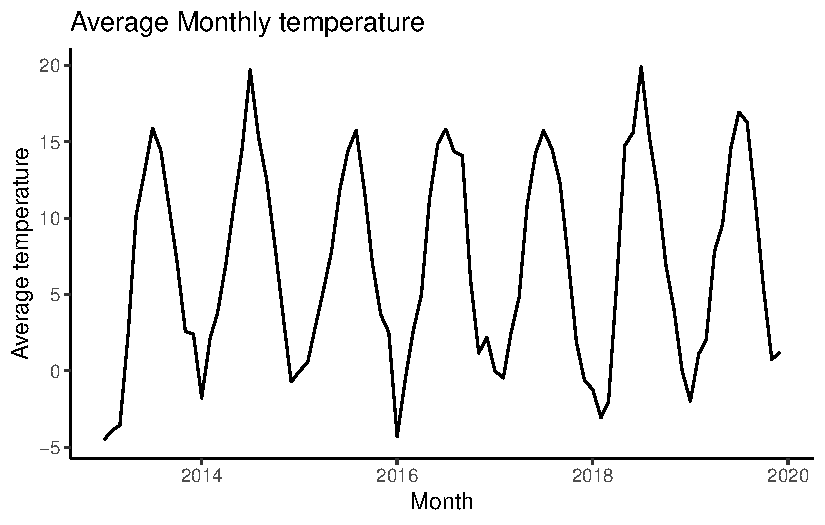
\includegraphics{Assignment2_files/figure-pdf/unnamed-chunk-5-1.pdf}

}

\end{figure}

As expected we see variations in average temperatures between the
seasons. We notice that the lowest temperatures are recorded during
winter and the highest during summers. Also, we notice that the min. and
max. temperatures are relatively equal each year.

We can also comment on the plot of monthly averages in volume.

\begin{Shaded}
\begin{Highlighting}[]
\CommentTok{\# Plot monthly average volume}
\NormalTok{plot\_list}\SpecialCharTok{$}\NormalTok{volume}
\end{Highlighting}
\end{Shaded}

\begin{figure}[H]

{\centering 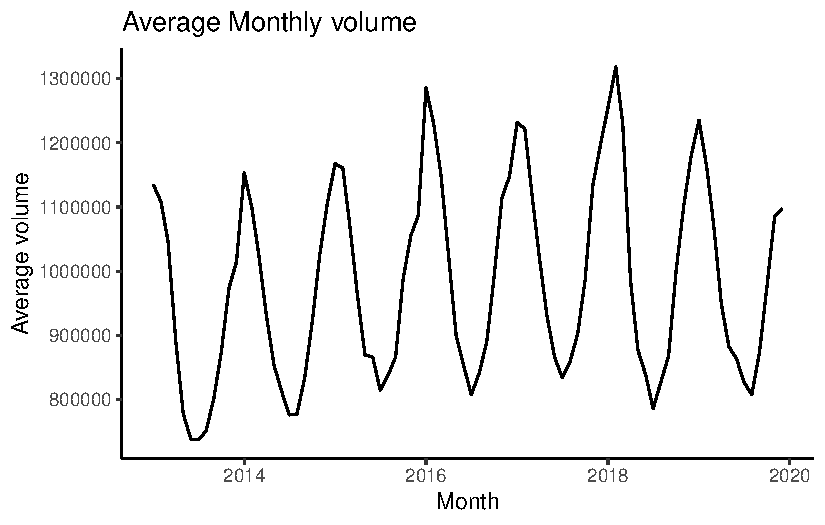
\includegraphics{Assignment2_files/figure-pdf/unnamed-chunk-6-1.pdf}

}

\end{figure}

In the plot we se that the energy consumption is is at max during winter
and are lowest during winters. There are also differences between
different year, but no great differences.

The next plot to examine is the plot of monthly averages of price.

\begin{Shaded}
\begin{Highlighting}[]
\CommentTok{\# Plot monthly average price}
\NormalTok{plot\_list}\SpecialCharTok{$}\NormalTok{price}
\end{Highlighting}
\end{Shaded}

\begin{figure}[H]

{\centering 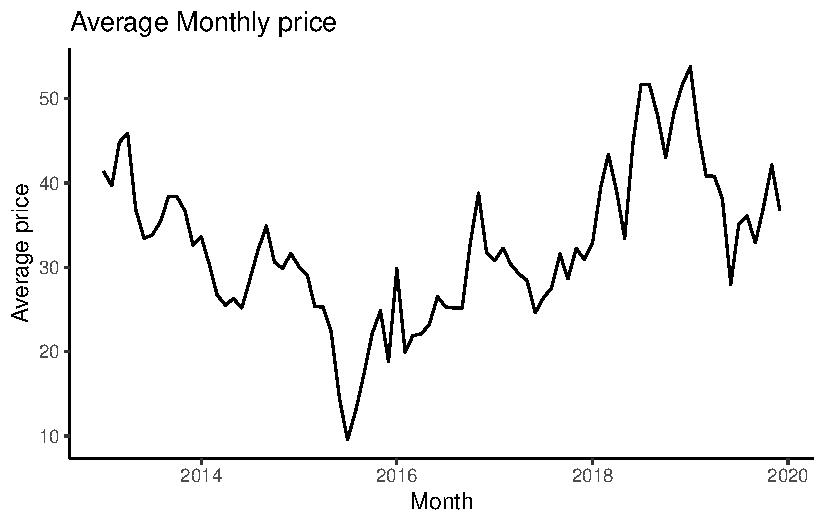
\includegraphics{Assignment2_files/figure-pdf/unnamed-chunk-7-1.pdf}

}

\end{figure}

We notice some seasonal trends in the prices of energy, however, the
biggest variations is betwween years. W notice a substantial dip in
energy prices during the summer of 2015, however the price continued to
rise up until the winter of 2019. After that it has returned to
2018-levels.

The last single plot to examine is the plot of monthly wind production.

\begin{Shaded}
\begin{Highlighting}[]
\CommentTok{\# Plot monthly average wind production}
\NormalTok{plot\_list}\SpecialCharTok{$}\NormalTok{wind\_production. }
\end{Highlighting}
\end{Shaded}

\begin{verbatim}
NULL
\end{verbatim}

Also in this plot we notice seasonal variations with highs during
autumn/winter and lows during summer.

Lastly, we can examine the relationship between the different variables.

\begin{Shaded}
\begin{Highlighting}[]
\CommentTok{\# Create a function that handles multiple variables and creates single plot}
\NormalTok{plot\_avg\_monthly\_multi }\OtherTok{\textless{}{-}} \ControlFlowTok{function}\NormalTok{(data, variables) \{}
  
  \CommentTok{\# Check if the specified variable is valid}
  \ControlFlowTok{if}\NormalTok{ (}\FunctionTok{all}\NormalTok{(variables }\SpecialCharTok{\%in\%} \FunctionTok{names}\NormalTok{(data))) \{}
    
    \CommentTok{\# Extract year and month, calculate the average per month of both variables}
\NormalTok{    avg\_data }\OtherTok{\textless{}{-}}\NormalTok{ data }\SpecialCharTok{\%\textgreater{}\%}
      \FunctionTok{mutate}\NormalTok{(}\AttributeTok{year\_month =} \FunctionTok{floor\_date}\NormalTok{(date, }\StringTok{"month"}\NormalTok{)) }\SpecialCharTok{\%\textgreater{}\%}
      \FunctionTok{group\_by}\NormalTok{(year\_month) }\SpecialCharTok{\%\textgreater{}\%}
      \FunctionTok{summarise}\NormalTok{(}\AttributeTok{avg\_var1 =} \FunctionTok{mean}\NormalTok{(}\FunctionTok{get}\NormalTok{(variables[}\DecValTok{1}\NormalTok{]), }\AttributeTok{na.rm =} \ConstantTok{TRUE}\NormalTok{),}
                \AttributeTok{avg\_var2 =} \FunctionTok{mean}\NormalTok{(}\FunctionTok{get}\NormalTok{(variables[}\DecValTok{2}\NormalTok{]), }\AttributeTok{na.rm =} \ConstantTok{TRUE}\NormalTok{), }
                \AttributeTok{.groups =} \StringTok{"drop"}\NormalTok{)}
    
    \CommentTok{\# Compute a scaling factor to map both variables onto a similar scale}
\NormalTok{    scale\_factor }\OtherTok{\textless{}{-}} \FunctionTok{mean}\NormalTok{(avg\_data}\SpecialCharTok{$}\NormalTok{avg\_var1, }\AttributeTok{na.rm =} \ConstantTok{TRUE}\NormalTok{) }\SpecialCharTok{/} 
                    \FunctionTok{mean}\NormalTok{(avg\_data}\SpecialCharTok{$}\NormalTok{avg\_var2, }\AttributeTok{na.rm =} \ConstantTok{TRUE}\NormalTok{)}
    
    \CommentTok{\# Plot}
\NormalTok{    p }\OtherTok{\textless{}{-}} \FunctionTok{ggplot}\NormalTok{(avg\_data, }\FunctionTok{aes}\NormalTok{(}\AttributeTok{x =}\NormalTok{ year\_month)) }\SpecialCharTok{+}
      \FunctionTok{geom\_line}\NormalTok{(}\FunctionTok{aes}\NormalTok{(}\AttributeTok{y =}\NormalTok{ avg\_var1), }\AttributeTok{color =} \StringTok{"red"}\NormalTok{) }\SpecialCharTok{+}
      \FunctionTok{geom\_line}\NormalTok{(}\FunctionTok{aes}\NormalTok{(}\AttributeTok{y =}\NormalTok{ avg\_var2 }\SpecialCharTok{*}\NormalTok{ scale\_factor), }\AttributeTok{color =} \StringTok{"blue"}\NormalTok{, }\AttributeTok{linetype =} \StringTok{"dashed"}\NormalTok{) }\SpecialCharTok{+}
      \FunctionTok{scale\_y\_continuous}\NormalTok{(}
        \AttributeTok{name =} \FunctionTok{paste}\NormalTok{(}\StringTok{"Average"}\NormalTok{, variables[}\DecValTok{1}\NormalTok{]),}
        \AttributeTok{sec.axis =} \FunctionTok{sec\_axis}\NormalTok{(}\SpecialCharTok{\textasciitilde{}}\NormalTok{. }\SpecialCharTok{/}\NormalTok{ scale\_factor, }\AttributeTok{name =} \FunctionTok{paste}\NormalTok{(}\StringTok{"Average"}\NormalTok{, variables[}\DecValTok{2}\NormalTok{])),}
        \AttributeTok{labels =}\NormalTok{ scales}\SpecialCharTok{::}\NormalTok{number}
\NormalTok{      ) }\SpecialCharTok{+}
      \FunctionTok{labs}\NormalTok{(}
        \AttributeTok{x =} \StringTok{"Month"}\NormalTok{,}
        \AttributeTok{title =} \FunctionTok{paste}\NormalTok{(}\StringTok{"Monthly averages of"}\NormalTok{, }\FunctionTok{paste}\NormalTok{(variables, }\AttributeTok{collapse =} \StringTok{" \& "}\NormalTok{))}
\NormalTok{      ) }\SpecialCharTok{+}
      \FunctionTok{theme\_classic}\NormalTok{()}
    \FunctionTok{return}\NormalTok{(p)}
    
  \CommentTok{\# If the specified variable is invalid  }
\NormalTok{  \} }\ControlFlowTok{else}\NormalTok{ \{}
    \FunctionTok{stop}\NormalTok{(}\StringTok{"Invalid variable name. Choose variables present in the data frame."}\NormalTok{)}
\NormalTok{  \}}
\NormalTok{\}}
\end{Highlighting}
\end{Shaded}

\begin{Shaded}
\begin{Highlighting}[]
\CommentTok{\# Plot relationship between variables}

\CommentTok{\# Initialize empty list}
\NormalTok{plot\_list\_multi }\OtherTok{\textless{}{-}} \FunctionTok{list}\NormalTok{()}

\CommentTok{\# Loop over variables and store comparison plots in list}
\ControlFlowTok{for}\NormalTok{ (i }\ControlFlowTok{in} \DecValTok{1}\SpecialCharTok{:}\NormalTok{(}\FunctionTok{length}\NormalTok{(variable\_list) }\SpecialCharTok{{-}} \DecValTok{1}\NormalTok{)) \{}
  \ControlFlowTok{for}\NormalTok{ (j }\ControlFlowTok{in}\NormalTok{ (i }\SpecialCharTok{+} \DecValTok{1}\NormalTok{)}\SpecialCharTok{:}\FunctionTok{length}\NormalTok{(variable\_list)) \{}
\NormalTok{    current\_vars }\OtherTok{\textless{}{-}} \FunctionTok{c}\NormalTok{(variable\_list[i], variable\_list[j])}
\NormalTok{    p }\OtherTok{\textless{}{-}} \FunctionTok{plot\_avg\_monthly\_multi}\NormalTok{(df, current\_vars)}
\NormalTok{    plot\_name }\OtherTok{\textless{}{-}} \FunctionTok{paste}\NormalTok{(current\_vars, }\AttributeTok{collapse =} \StringTok{"\_vs\_"}\NormalTok{)}
\NormalTok{    plot\_list\_multi[[plot\_name]] }\OtherTok{\textless{}{-}}\NormalTok{ p}
\NormalTok{  \}}
\NormalTok{\}}
\end{Highlighting}
\end{Shaded}

Comparing the four specified variables adds up to six comparison plots.
We chose only to discuss the three most relevant, temperature vs.~volume
and price vs.~volume. Notice that to compare the variables, we have
added a second axis to each plot since the variables have different
scales. In some cases, like the temperature vs.~volume plot, this has
lead to some errors. Errors like this is easy to spot if you compare
with the single variable plot. Despite the scaling errors we chose to
include them since they visualize relationships between the variables.

The first plot we examine is the temperature vs.~volume plot.

\begin{Shaded}
\begin{Highlighting}[]
\CommentTok{\# Compare temperature vs. volume}
\NormalTok{plot\_list\_multi}\SpecialCharTok{$}\NormalTok{temperature\_vs\_volume}
\end{Highlighting}
\end{Shaded}

\begin{figure}[H]

{\centering 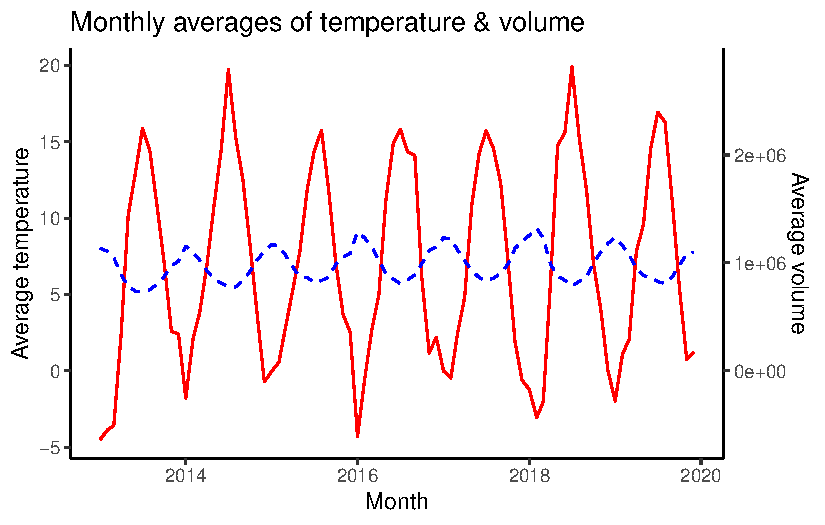
\includegraphics{Assignment2_files/figure-pdf/unnamed-chunk-11-1.pdf}

}

\end{figure}

Despite the errors in scaling, we notice that when temperatures
increases, the volume decrease and vice versa.

The second plot of interest is the volume vs.~price plot.

\begin{Shaded}
\begin{Highlighting}[]
\NormalTok{plot\_list\_multi}\SpecialCharTok{$}\NormalTok{volume\_vs\_price}
\end{Highlighting}
\end{Shaded}

\begin{figure}[H]

{\centering 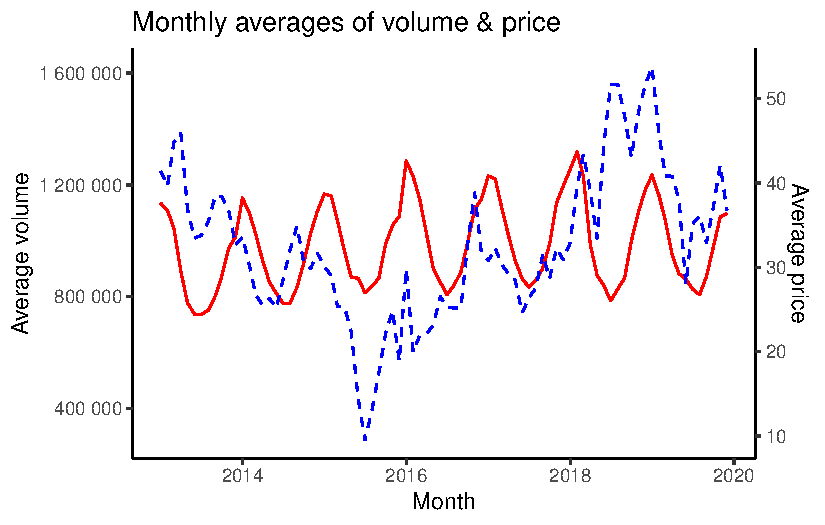
\includegraphics{Assignment2_files/figure-pdf/unnamed-chunk-12-1.pdf}

}

\end{figure}

We notice the at times close relationship of the two variables. In
periods of high volume, the price tends to be relativly high and vice
versa. This is likely due to a energy surplus in periods with low demand
resulting in low prices, and increased prices in periods of high demand.

\hypertarget{task-b.-why-will-a-ols-regression-on-quantity-not-provide-an-estimate-of-demand}{%
\subsection{Task B. Why will a OLS regression on quantity not provide an
estimate of
demand?}\label{task-b.-why-will-a-ols-regression-on-quantity-not-provide-an-estimate-of-demand}}

An OLS regression of quantity on price alone, even with controls, is not
fitted to estimate demand due to many reasons:

\begin{enumerate}
\def\labelenumi{\arabic{enumi}.}
\item
  Endogeneity exists as price and quantity in markets are simultaneously
  determined
\item
  Omitted variables like for example consumer income, advertising and
  seasonality. These can affect and lead to omitted variable bias.
\item
  Measurement errors in price and quantity can contribute to bias for
  the estimates for the parameters
\item
  OLS (or Gauss-Markow theorem) assumes a linear relationship. This may
  not hold if the demand curves are nonlinear.
\item
  Heteroskedasticity which is variability in the error term given any
  explanatory variable. In this case the variability in quantity varies
  across price levels which in return can affect standard erros.
\item
  The demand's dynamic behavior and seasonality may not be sufficiently
  captured. To estimate demand accurately, more advanced econometric
  methods are often required. These advanced methods usually contain
  instrumental variable regression and structural equation modelling.
  Controlling for relevant factors and improve our data quality can also
  make the estimation precision better.
\end{enumerate}

\hypertarget{task-c.-considering-choice-of-instrument-for-price-when-estimating-demand}{%
\subsection{Task C. Considering choice of instrument for price when
estimating
demand}\label{task-c.-considering-choice-of-instrument-for-price-when-estimating-demand}}

When choosing a instrument for price when estimating demand, it's
important to consider the validity of the instrument in terms of the
requirements for a valid instrument. These requirements can be
relevance, exogeneity, and exclusion restrictions:

\begin{enumerate}
\def\labelenumi{\arabic{enumi}.}
\item
  Why is temperature not a valid instrument for price when estimating
  demand? The key requirements for exogeneity may not be satisfied if
  one were to use temperature as an instrument for price when estimating
  demand. (Exogeneity refers to the condition in which an independent
  variable is unrelated to the error term, indicating that it is not
  influenced by unobserved factors in the model.) Temperature is usually
  affected by factors that also may affect demand, like seasonality and
  consumber behavior. The instrument would not be valid due to
  endogeneity concerns if temperature is correlated with unobservable
  demand shocks.
\item
  Why can magazine levels (or deviations) and wind power production
  potentially be good instruments for price when estimating demand?
  Magazine levels and wind power production could potentially be
  sufficient instruments for price as they can fulfil the requirements
  for a valid instrument. They should be relevant in other terms they
  should be affecting the price. In addition, they should be exogenous,
  meaning that they should not be correlated with unobservable factors.
  But establishing their exogeneity requires thoughtful consideration
  and testing.
\item
  Why is it necessary to control for seasonality (say, calendar month)
  and temperature? It is necessary to control for seasonality and
  temperature to avoid omitted variable bias. (Omitted variable bias
  appear if a relevant variable that affects the dependent variable is
  excluded in a regression model. This leads to biased and estimates of
  the coefficients of the variables that are included.) Seasonality
  captures variation in the systematic demand throughout the year
  unrelated to price. Meanwhile temperature affects demand
  independently. When we control for these factors, we ensure precise
  demand estimates.
\item
  How could controlling for weekday and year be useful? Incorporating
  controls for weekday and year is beneficial to justify for demand
  patterns variation. Weekdays and weekends usually give different
  demand profiles given the consumers consumption. Meanwhile years would
  capture trends that are long-term and macroeconomic affects on demand.
  These controls strengthen the accuracy of demand estimates, while
  taking into account sources of variation unrelated to price.
\end{enumerate}



\end{document}
